
\subsection{A plausible (but bad) alternative}
\label{sec:dt}


The MIP models generated by \sys can grow large as the sizes of the
data and the log increase. However, modeling all present constraints
from the beginning to the end of the log is necessary; in this
section, we examine alternative, simpler models that process a single
query at a time, and demonstrate why they are insufficient.

\smallskip
\noindent
\textbf{WHERE repairs through classification:}
The \texttt{WHERE} clause of an update query is equivalent to a
rule-based binary classifier that splits tuples into two groups:
(1)~tuples that satisfy the conditions in the \texttt{WHERE} clause
and (2)~tuples that do not. A mistake in a query predicate can then
result in misclassification: some tuples get classified into the wrong
group, which in turn translates to errors in the data. Therefore,
repairing the mistake corresponds to repairing the imprecise
classification. This works as follows: For an incorrect query $q$, let
$D_0$ be the database state before $q$, and $D_1^*$ the \emph{correct}
database state that should result after $q$.
We use each tuple $t \in D_0$ as an element in the input training data
for the classifier where the values (of each attribute) of $t$ define
the feature vector and the label for $t$:
	\[
    label(t)= 
    \begin{cases}
    true ,& D_0.t \neq D_1^*.t\\
    false,              & \text{otherwise}
    \end{cases}
\]
We then train a classifier, such as decision trees \cite{???} to learn
the correct classification rules rules for the \texttt{WHERE} clause.


\smallskip
\noindent
\textbf{SET repairs:}
After repairing the \texttt{WHERE} clause through learning a
rule-based classifier, some complaints may still persist. This
indicates a possible error in the \texttt{SET} clause. The errors can
be modeled and solved by constructing a simple linear system of
equations: For each expression in the \texttt{SET} clause we create a
linear equation, using unknown variables to represent any parameters
in the \texttt{SET} expression. Solving for these variables then
provides a repair for the \texttt{SET} expression.


\smallskip
\noindent
\textbf{Why it does not work:}
The na\"ive approach that we just described is heuristic in nature. It
is simple and fast, but it can only process a single incorrect query.
This results in several shortcomings that make it insufficient in
practice:
\begin{itemize}[itemsep=1pt, leftmargin=5mm]
    
\item In principle, one could attempt to apply this technique to the
entire log one-query-at-a-time. However, this is not possible in
practice: to learn a classifier on the \texttt{WHERE} clause of query
$q_i$, one needs to know the correct classification output, which
corresponds to $D_i^*$. Unfortunately, even with a complete complaint
set, which can derive the correct database $D_n^*$, there is no
obvious way to ``rollback'' this state to derive $D_i^*$.

\item The classifier may derive a clause that is structurally very
different from the original one (different attributes or number of
conditions). This is problematic in general, as it corresponds to a
larger-scale mistake in the query, which is a less likely scenario.

\item Classifiers try to avoid overfitting, which is problematic for
queries with high selectivity (e.g., single-tuple updates), as the
classifier is unlikely to generate any rules.

\end{itemize}


Therefore, while examining one query at a time superficially appears
to be a reasonable and efficient alternative, the reality is that one
has to model all constraints and transformations through the entire
log history. In the following section, we propose several
optimizations to our initial approach that make scaling to large data
and log sizes feasible. 


\iffalse
In this
section, we examine alternative, simpler models that process a single
query at a time, and demonstrate why they are insufficient.

\noindent
\textbf{WHERE repairs through classification:}
The \texttt{WHERE} clause of an update query is equivalent to a
rule-based binary classifier that splits tuples into two groups:
(1)~tuples that satisfy the conditions in the \texttt{WHERE} clause
and (2)~tuples that do not. Thus, by training a classifier,
such as decision trees \cite{quinlan1987} to learn
the correct classification rules rules for the \texttt{WHERE} clause.

\noindent
\textbf{SET repairs:}
This alternative approach constructs 
a simple linear system of equations to solve the parameters in the \texttt{SET}
when errors persist after fixing the \texttt{WHERE} clause:
For each expression in the \texttt{SET} clause we create a
linear equation, using unknown variables to represent any parameters
in the \texttt{SET} expression. 
  \begin{figure}[h]
  \centering
    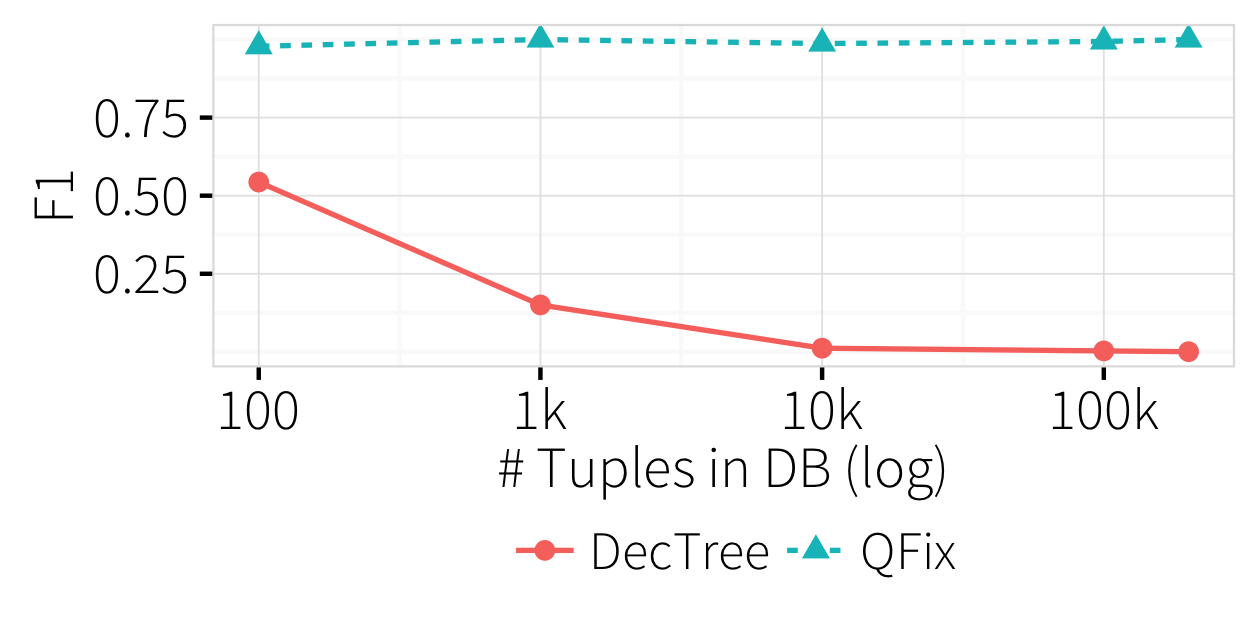
\includegraphics[width = .6\columnwidth]{figures/heuristicacc}
    \vspace*{-.1in}
    \caption{Heuristic Approach vs. \sys on Single-Query. }
    \label{f:heuristic_acc} 
  \end{figure}
  \vspace*{-0.1in}
  
The na\"ive approach that we just described is heuristic in nature. It
is simple and fast, but it can only process a single incorrect query. As shown in
Figure~\ref{f:heuristic_acc}, the F-1 score of na\"ive heuristic approach is less 
than 0.6 while \sys maintain high accuracy in solving single query problem with
above 0.9 F-1 score across all database sizes. 
\fi
